\section{Detector-level results}
\label{sec:m4lrecoresults}
In this section the detector-level selected events are presented and compared to the SM predictions for the single $Z$, Higgs, \onshellZZ and \offshellZZ mass regions, and for the inclusive \mFourL{} distribution. The reducible background described in Section~\ref{sec:background} is also included. 

The number of selected events in the four \mFourL{} regions over the full fiducial phase space is presented in Table~\ref{tab:RecoYieldTablePerProcess}, along with the predicted number of events, and the predicted background contribution from non-prompt leptons. For the \qqFourL{} process the \SHERPA{} simulation is used. The combined uncertainties (systematic and statistical) are also quoted. The uncertainty in the total prediction takes into account correlations between processes, and therefore contributions in a given column do not trivially add up in quadrature to give the total. Uncertainties in the predictions arise from the sources discussed in Sections~\ref{sec:background} and~\ref{sec:uncertainties}. 

\begin{table}
    \centering    
    \caption{Predicted reconstruction-level yields per process and in total,
      compared with observed data counts, over the full fiducial phase space and in the
      following regions of
      $\mFourL$: \ZFourL{}  ($60 < \mFourL < 100$~\GeV), \HFourL{}  ($120 <
\mFourL < 130$~\GeV), off-shell $\Z\Z$  ($20 <
\mFourL < 60$~\GeV\ or $100 <
\mFourL < 120$~\GeV\ or $130 <
\mFourL < 180$~\GeV) and  on-shell \Z\Z{} ($180 <
\mFourL < 2000$~\GeV).
     The background row is events with non-prompt leptons,
     including those from $\Z{} + \Upsilon{}$ events.
      The \HFourL{} row includes only the
      on-shell Higgs boson contribution, with off-shell contributions included in
     \ggFourL{}. \label{tab:RecoYieldTablePerProcess} }
  \begin{tabular} {l  c  c  c  c  c }
 \hline 
  & \multicolumn{5}{c}{Region} \\
      & Full   & \ZFourL{}  & \HFourL{}  & Off-shell $\Z\Z$  & On-shell $\Z\Z$   \\

 \hline 
\qqFourL{} & $6100 \pm 500$  & $1490 \pm 120$  & $128 \pm 10$  & $800 \pm 60$  & $3640 \pm 280$ \\
\ggFourL{} & $680 \pm 90$  & $10.8 \pm 2.9$  & ~~$3.9 \pm 0.7$  & $49 \pm 6$  & $620 \pm 80$ \\
\HFourL{}  & $245 \pm 20$  & ~~$2.16 \pm 0.18$  & $207 \pm 17$  & $33.5 \pm 3.1$  & $1.98 \pm 0.20$ \\
\V\V\V{}  & $35 \pm 4$  & ~~$0.018 \pm 0.005$  & ~~$0.127 \pm 0.018$  & ~~$2.05 \pm 0.22$  & $32.9 \pm 3.4$ \\
$t\bar{t}$\V(\V) & $123 \pm 19$  & ~~$1.37 \pm 0.22$  & ~~$1.2 \pm 0.2$  & $15.5 \pm 2.4$  & $105 \pm 16$ \\
Background & $330 \pm 50$  & $44 \pm 8$  & $26 \pm 5$  & $129 \pm 19$  & $139 \pm 30$ \\    
\hline 
Total Pred. & $7500 \pm 500$  & $1540 \pm 110$  & $367 \pm 19$  & $1030 \pm 60$~~  & $4530 \pm 290$ \\
\hline 
Data & $7755 $  & $1452 $  & $379 $  & $1095 $  & $4828 $ \\
 \hline 
 \end{tabular}
\end{table}

Figure~\ref{fig:recoresults1} shows the inclusive \mFourL{} distribution at the detector level. The data are plotted in black along with the uncertainties. The SM prediction is separated into the individual dominant processes described in Section~\ref{sec:fourlepmotivation} and plotted as stacked histograms. 
Overall the data are in good agreement with the predictions, with some minor fluctuations in the high mass bins due to low statistics. The detector-level plots for the rest of the observables are not shown in the scope of this thesis, but are published in Reference~\cite{m4l2021_paper}. 
\begin{figure}[htb]
\centering
 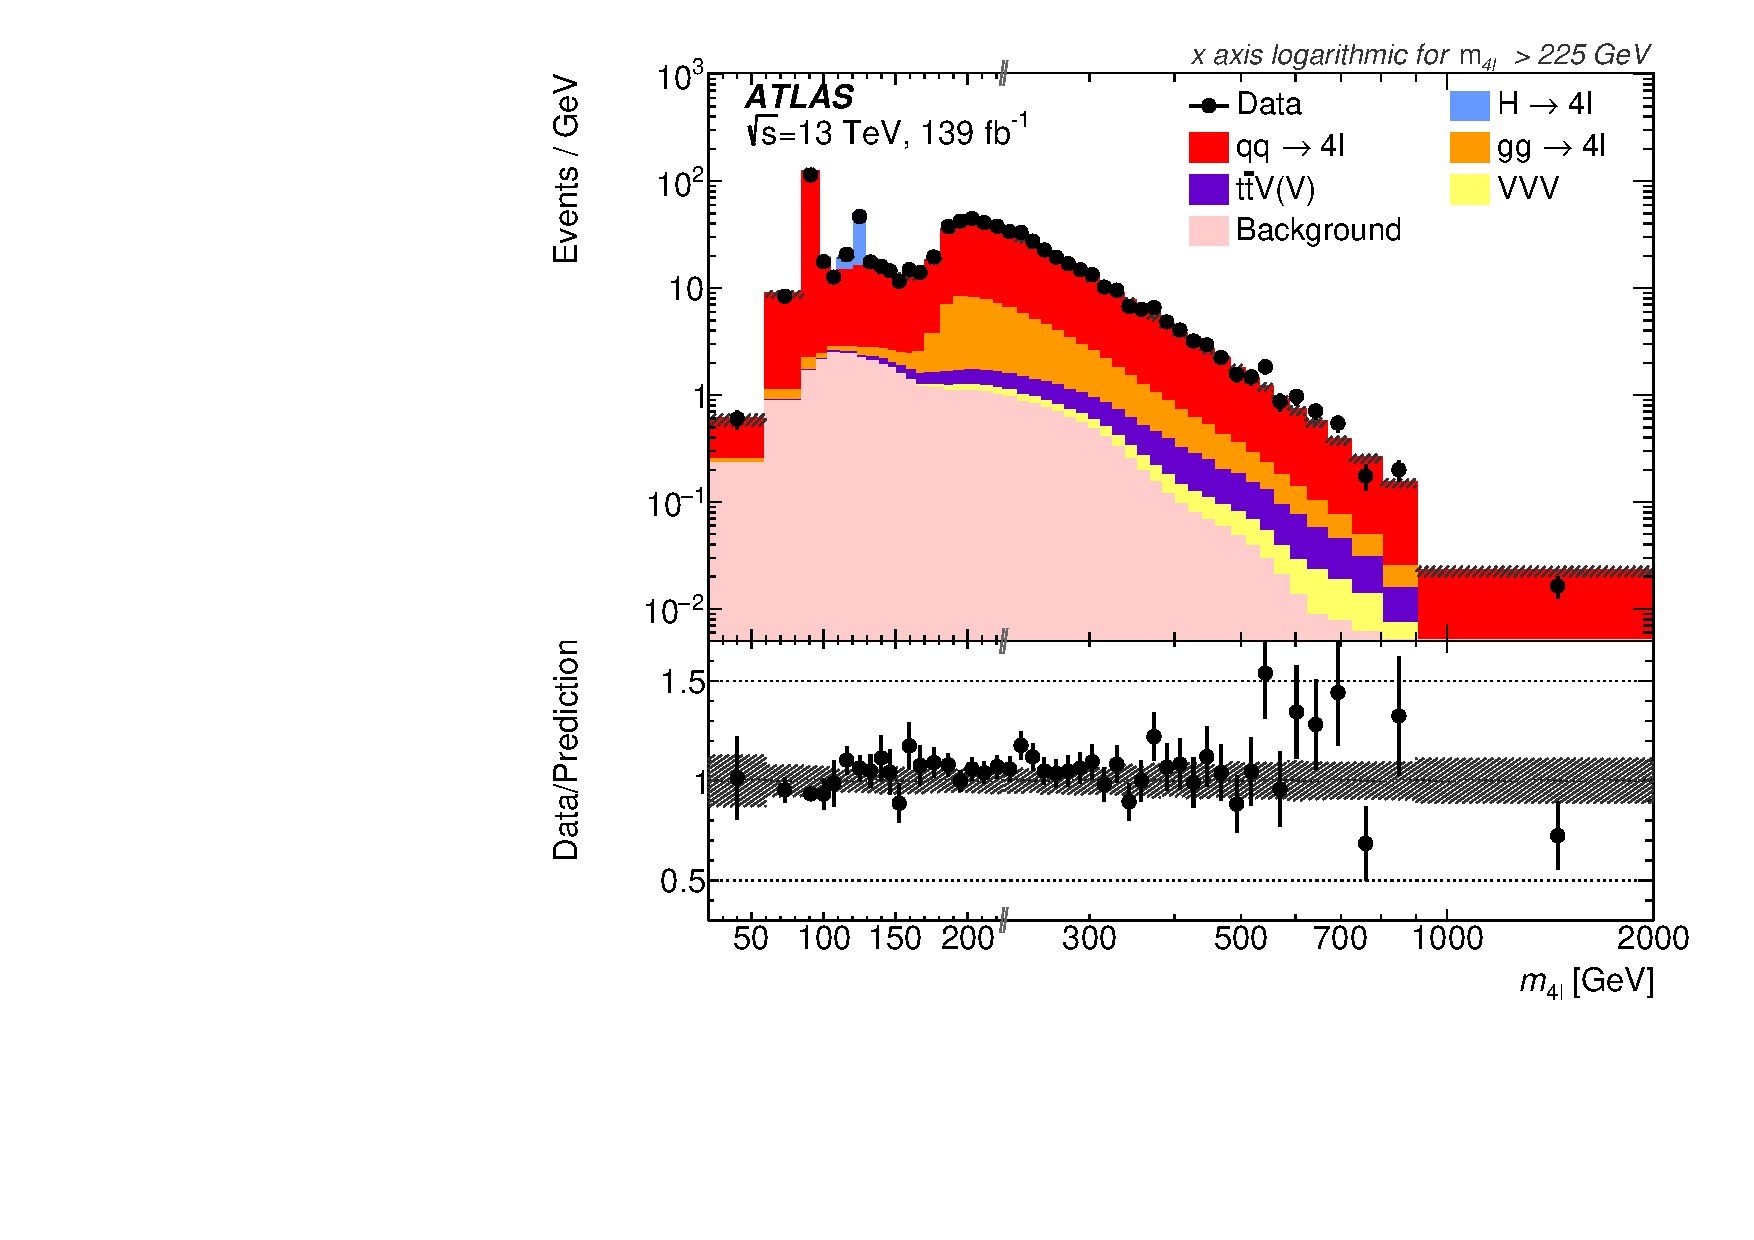
\includegraphics[width = 0.7\textwidth]{Figures/m4l/Overlay_M4l_0__forPaper.pdf}
    \caption{Observed reconstruction-level \mFourL{} distribution compared with the SM prediction, using
      \SHERPA{} for the \qqFourL{} simulation.
     The statistical uncertainty of the
      data is displayed as error bars and systematic uncertainties
      in the prediction are shown as a grey hashed band.  The
      ratio of the data to the prediction is shown in the lower
      panel.  The $x$-axis is on a linear scale until $\mFourL = 225$~\GeV,
where it switches to a logarithmic scale, as indicated by the double
dashes on the axis.
      There is one additional data event reconstructed with 
$\mFourL = 2.14$~\TeV, while 0.4 events are expected from simulation for
$\mFourL > 2$~\TeV. This figure is from Ref.~\cite{m4l2021_paper}. \label{fig:recoresults1}}
\end{figure}
